\section{TDOA positioning in a plane}
\label{tdoaPositioning}
In this section the relationship between differences in time measurements from multiple sensors and the xy-position of the emitter are derived.
The problem can be modeled as in figure \ref{fig:tdoa_model} where the following parameters are known from the setup and measurements:
\begin{itemize}
	\item Time of arrival of sound at sensors a, b, c and d.
	\item Speed of sound in chosen material.
	\item Position of sensors.
\end{itemize}
The system is setup with four sensors since the possibility of resulting in multiple solutions when using only three \cite{tdoa_book}
The solution will be represented as a system of linear equations to enable fast and relatively simple implementation in VHDL.
The derivation will be conducted for two of the sensors giving one row in the equation system. The other two rows are determined in a similar manner.
\begin{figure}[htb]
	\centering
	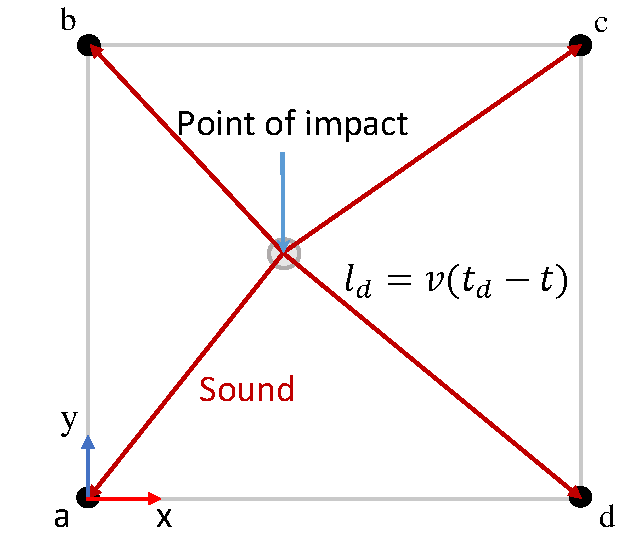
\includegraphics[width=.6\textwidth]{figures/tdoa_model}
	\caption{Side view of the platform surface area and the net. The red markings are piezoelectric sensors.}
	\label{fig:tdoa_model}
\end{figure}

By assuming a constant speed of sound through the impact plane, equation \ref{eq:speedOfSoundDistA} describes the relationship between time difference between measurement and impact $(t_a - t)$ and the distance the impact point is from sensor a.
\begin{equation}
	l_a = v(t_a - t) \Leftrightarrow l_a^2 = v^2(t_a - t)^2 
	\label{eq:speedOfSoundDistA}
\end{equation}
Equation \ref{eq:speedOfSoundDistB} describes the same relationship with respect to sensor b. 
\begin{equation}
	l_b = v(t_b - t) \Leftrightarrow l_b^2 = v^2(t_b - t)^2
\label{eq:speedOfSoundDistB}
\end{equation}
By differencing equation \ref{eq:speedOfSoundDistA} and \ref{eq:speedOfSoundDistB} equation \ref{eq:distanceDiffRelativeToTime} can be derived using the difference of squares formula. It is a linear relation with respect to time of impact $t$.
\begin{equation}
	l_a^2 - l_b^2 = v^2(t_a^2 - t_b^2) - 2 v^2 (t_a - t_b) t
	\label{eq:distanceDiffRelativeToTime}
\end{equation} 
By using Pythagoras theorem the difference in squared distances from the impact point are also related according to equation \ref{eq:distDifference}. It can be seen that it is a linear equation in x and y with constants given from the setup.
\begin{equation}
	\begin{split}
		l_a^2 - l_b^2 & = (x_a - x_b)^2 + (y_a - y)^2 - ((x_b-x)+(-y_b - y))^2 \\
		& = -2( (x_a - x_b) x + (y_a - y_b) y ) + x_a^2 +y_a^2 -(x_b^2 + y_b^2)
	\end{split}
	\label{eq:distDifference}
\end{equation}
By setting equation \ref{eq:distanceDiffRelativeToTime} and \ref{eq:distDifference} equal and isolating the constants known from time measurements and setup equation \ref{eq:firstRow} is derived.
\begin{equation}
	(x_a - x_b) x + (y_a - y_b) y - v^2(t_a - t_b) t = (x_a^2 +y_a^2 -(x_b^2 + y_b^2) - v^2(t_a^2 - t_b^2))/2 \equiv k_{ab}
	\label{eq:firstRow}
\end{equation}
Using similar relations for the other four sensors results in the system of linear equations \ref{eq:linsys} which solution uniquely defines the xy-position of the impact \cite{toa_notes}.
\begin{equation}
	\begin{bmatrix} 
		x_a - x_b & y_a - y_b & - v^2(t_a - t_b) \\
		x_b - x_c & y_b - y_c & - v^2(t_b - t_c) \\
		x_c - x_d & y_c - y_d & - v^2(t_c - t_d) 
	 \end{bmatrix}
	 \left[ \begin{array}{c} x \\ y \\ t \end{array} \right] = \left[ \begin{array}{c} k_{ab} \\ k_{bc} \\ k_{cd}\end{array} \right] 
	 \label{eq:linsys}
\end{equation}